\documentclass[11pt, addpoints, answers]{exam}

\usepackage{amsmath, amssymb, amsthm}
\usepackage{xcolor}
\usepackage{graphicx}
\usepackage{graphics}
\usepackage{tikz}
\usepackage{tikz-qtree}
\usetikzlibrary{graphs}
\tikzset{every tree node/.style={minimum width=2em,draw,circle},
    blank/.style={draw=none},
    edge from parent/.style=
    {draw,edge from parent path={(\tikzparentnode) -- (\tikzchildnode)}},
    level distance=1.2cm}
\usepackage{listings}   
\usepackage{caption}
\usepackage{algorithm}
\usepackage{algorithmicx}
\usepackage{algpseudocode}
\usepackage{underscore}
% \usepackage[top=2cm, bottom=2cm, left=2cm, right=2cm]{geometry}  
\makeatletter
\newcommand\dlmu[2][2.5cm]{\hskip1pt\underline{\hb@xt@ #1{\hss#2\hss}}\hskip3pt}
\makeatother

% For inserting code snippets.
\usepackage{listings}
\lstset{
    columns = fixed,
    basewidth = {0.5em},
    breaklines = true,
    backgroundcolor = \color{white},
    keywordstyle = \color[RGB]{40, 40, 255},
    numberstyle = \footnotesize\color{darkgray},
    commentstyle = \ttfamily\color{violet},
    basicstyle = \ttfamily,
    stringstyle = \ttfamily\color[RGB]{128, 0, 0},
    showstringspaces = false,
    language = {[11]C++},
    escapechar = \@
}
\lstnewenvironment{cpp}[1][]{\lstset{language = {[11]C++}, #1}}{}

\usepackage{tikz}

% headers, footers, titles
\newcommand{\CourseName}{CS101 Algorithms and Data Structures}
\newcommand{\HomeworkNO}{Homework 7}
\newcommand{\DueDate}{Due date: 23:59, October 26th, 2023}

\pagestyle{headandfoot}
\runningheadrule
\runningheader{\CourseName}{\HomeworkNO}{\DueDate}
\runningfooter{}{\thepage}{}

\title{
	\CourseName\\
	Fall 2023\\
	\HomeworkNO
}
\author{}
\date{\DueDate}

% formats of questions, choices, points, etc.
\qformat{\bf\thequestion. (\totalpoints\ points) \thequestiontitle\hfill}
\pointname{'}
\CorrectChoiceEmphasis{\bf\color{blue}}
\SolutionEmphasis{\color{blue}}

% We frequently use this font.
\newcommand{\ttt}{\texttt}

\begin{document}

\maketitle

\begin{enumerate}
	\item Please write your solutions in English.
	\item Submit your solutions to gradescope.com.
	\item Set your FULL name to your Chinese name and your STUDENT ID correctly in Account Settings.
	\item If you want to submit a handwritten version, scan it clearly. \ttt{CamScanner} is recommended.
	\item When submitting, match your solutions to the problems correctly.
	\item No late submission will be accepted.
	\item Violations to any of the above may result in zero points.
\end{enumerate}

\begin{questions}

\titledquestion{Multiple Choices}

Each question has \textbf{one or more} correct answer(s). Select all the correct answer(s). For each question, you will get 0 points if you select one or more wrong answers, but you will get 1 point if you select a non-empty subset of the correct answers.

Write your answers in the following table.

%%%%%%%%%%%%%%%%%%%%%%%%%%%%%%%%%%%%%%%%%%%%%%%%%%%%%%%%%%%%%%%%%%%%%%%%%%%
% Note: The `LaTeX' way to answer a multiple-choices question is to replace `\choice'
% with `\CorrectChoice', as what you did in the first question. However, there are still
% many students who would like to handwrite their homework. To make TA's work easier,
% you have to fill your selected choices in the table below, no matter whether you use 
% LaTeX or not.
%%%%%%%%%%%%%%%%%%%%%%%%%%%%%%%%%%%%%%%%%%%%%%%%%%%%%%%%%%%%%%%%%%%%%%%%%%%

\begin{table}[htbp]
    \centering
    \begin{tabular}{|p{2cm}|p{2cm}|p{2cm}|p{2cm}|p{2cm}|p{2cm}|}
        \hline
        (a) & (b) & (c) & (d) & (e) & (f) \\
        \hline
        %%%%%%%%%%%%%%%%%%%%%%%%%%%%%%%%%%%%%%%%%%%%%%%%%%%%%%%%%%
        % YOUR ANSWER HERE.
        &     &     &     &     &     \\
        %%%%%%%%%%%%%%%%%%%%%%%%%%%%%%%%%%%%%%%%%%%%%%%%%%%%%%%%%%
        \hline
    \end{tabular}\label{tab:multiple}
\end{table}

\begin{parts}
    \part[2] Which of the following statements is/are true about \textbf{tree}?

    \begin{choices}
        \choice A tree with $N$ nodes has $N-1$ edges.
        \choice The height of a tree is always positive.
        \choice Every node of a tree is either a leaf node or an internal node.
        \choice The degree and the depth of the root node should be $0$.
    \end{choices}

    \part[2] Which of the following statements is/are true about \textbf{binary tree}?

    \begin{choices}
        \choice In a binary tree, every non-root node has exactly one parent.
        \choice Every full binary tree is also a complete binary tree.
        \choice A full binary tree with $n$ non-leaf nodes contains $2n - 1$ total nodes.
        \choice A binary tree of height $0$ is also perfect.
    \end{choices}

    \part[2] Which of the following choices is/are $\Theta(m)$ where $m$ is the maximum length of the queue when traversing a tree with BFS?

    \begin{choices}
        \choice The total number of nodes in the tree.
        \choice The length of the deepest path from a leaf node to the root node.
        \choice The maximum degree of nodes in the tree.
        \choice The maximum number of nodes at a given depth of the tree.
    \end{choices}

    \part[2] There exists two paths between any two different nodes in a tree with height more than 3.

    \begin{choices}
        \choice True.
        \choice False.
    \end{choices}

    \part[2] The height of a tree is always equal to the maximum depth of nodes in the tree.

    \begin{choices}
        \choice True.
        \choice False.
    \end{choices}

    \part[2] Which of the following statements is/are false?

    \begin{choices}
        \choice Nodes with the same depth are siblings.
        \choice Each node in the tree has exactly one parent pointing to it.
        \choice Given any node $\alpha$ within a tree, the collection of $\alpha$ and all of its descendants is a subtree of the tree with root $\alpha$.
        \choice The root node cannot be the descendent of any nodes.
    \end{choices}

\end{parts}

\newpage

\titledquestion{AVL tree operations}

Here is an AVL tree. Denote it as $T$.
\begin{center}
    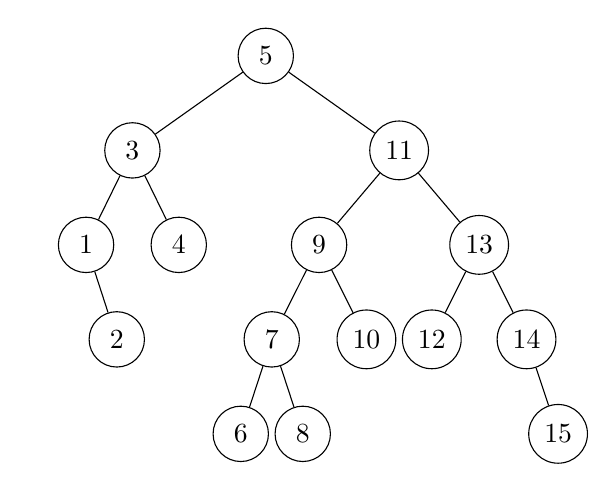
\begin{tikzpicture}[]
    \Tree
    [.5
        [.3
            [.1
                \edge[blank]; \node[blank]{};
                [.2
                ]
            ]
            [.4
            ]
        ]
        [.11
            [.9
                [.7
                    [.6
                    ]
                    [.8
                    ]
                ]
                [.10
                ]
            ]
            [.13
                [.12
                ]
                [.14
                    \edge[blank]; \node[blank]{};
                    [.15
                    ]
                ]
            ]
        ]
    ]
    \end{tikzpicture}
\end{center}

\begin{parts}

\part[2] Insert $8.5$ into $T$. Draw the AVL tree before checking if any balance correction is needed.

\vspace{7cm}

\part[2] Insert $8.5$ into $T$. Draw the AVL tree after balance corrections.

\vspace{7cm}

\part[2] Remove $3$ from $T$ (\textbf{NOT from the previous answer!}). Draw the AVL tree after replacing and before checking if any balance correction is needed.

\vspace{7cm}

\part[2] Remove $3$ from $T$. Draw the AVL tree after balance corrections.

\vspace{7cm}

\end{parts}


\end{questions}

\end{document}